\documentclass{article}
\usepackage[margin=2cm]{geometry}
\usepackage[utf8]{inputenc}
\usepackage{minted}
\usepackage{amsfonts}
\usepackage{amsmath}
\usepackage{tikz}
\usepackage{}

\title{CSC258 PRELAB 7}
\author{Tingfeng Xia}
\date{\today}

\usepackage{natbib}
\usepackage{graphicx}

\begin{document}

\maketitle
\section*{PART I}
\paragraph{(9)} I should first present my test cases, below is the writing that we will do. We will read from positions \texttt{00000}, \texttt{01000},\texttt{10000}, and \texttt{11100}. The first three are the three boxes to the top left of the memory block above, while the last one \texttt{11100} is 28 in binary, corresponding to the bottom right box.
\begin{center}
    \begin{tabular}{ ||cccc|cccc|| }
        \hline\hline
        0 & 0 & 0 & 1 & 0 & 0 & 0 & 0 \\ \hline
        0 & 0 & 1 & 0 & 0 & 0 & 0 & 0 \\ \hline
        0 & 0 & 1 & 1 & 0 & 0 & 0 & 0 \\ \hline
        0 & 1 & 0 & 0 & 0 & 0 & 0 & 0 \\
        \hline\hline
    \end{tabular}
\end{center}
Indeed, we have the following in the ModelSim results for the \texttt{ram32x4.v} module that we just created.
\begin{center}
    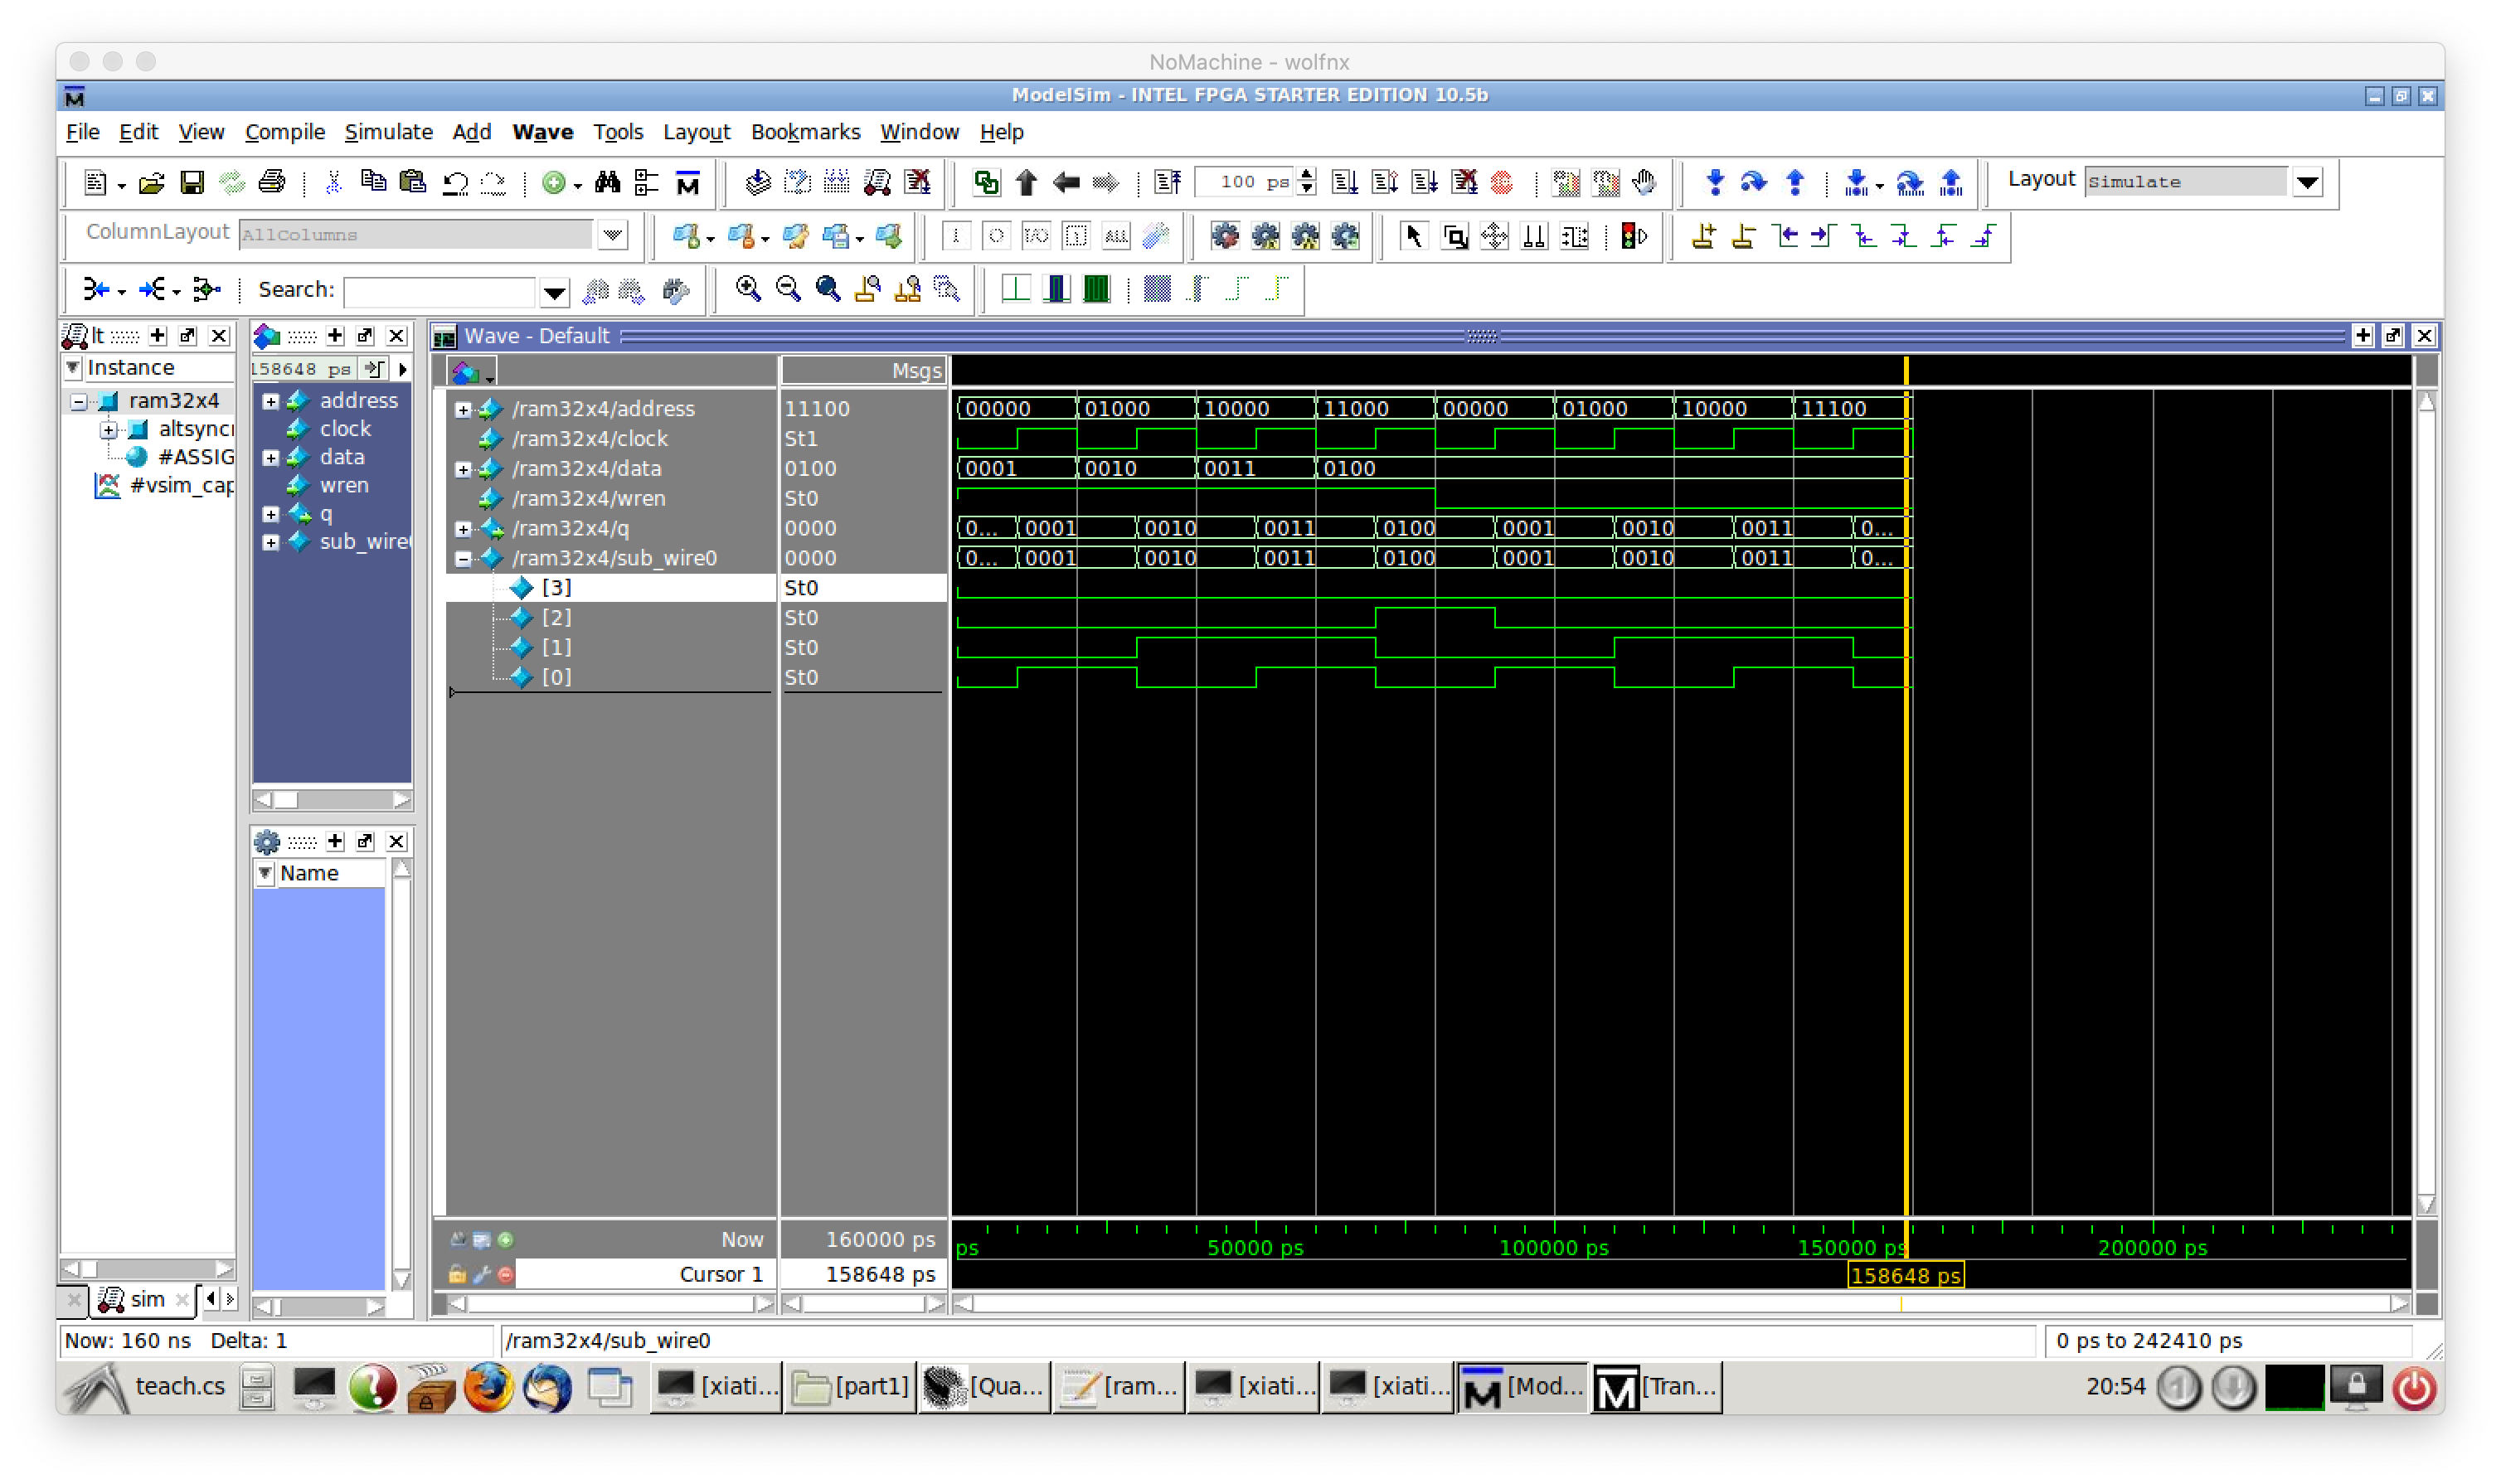
\includegraphics[scale=0.33]{part1_sim_ram32x4.png}
\end{center}

\paragraph{(10)} Here is my code that instantiates the \texttt{ram32x4.v} module from top level. Notice that this will only work if the \texttt{ram32x4.v} was included as part of the project. Here is my code

\begin{minted}{verilog}
    // SW[3:0] for data inputs
    // SW[8:4] for address inputs
    // SW[9] is write enable
    // KEY[0] clock
    
    // show address on HEX5 and HEX4
    // input data on HEX2
    // output data on HEX0 (output of memory)
    
    module ram_toplv(
            input [9:0] SW,
            input [0:0] KEY, 
            output [6:0] HEX5, 
            output [6:0] HEX4, 
            output [6:0] HEX2,
            output [6:0] HEX0
    );
        wire [3:0] ramout;
        
        ram32x4 ram_block(
            .address(SW[8:4]),
            .clock(KEY[0]),
            .data(SW[3:0]),
            .wren(SW[9]),
            .q(ramout[3:0])
        );
        
        // The last bit, for hex5
        hex_decoder hex5({3'b000, SW[8]}, HEX5[6:0]);
        hex_decoder hex4(SW[7:4], HEX4[6:0]);
        hex_decoder hex2(SW[3:0], HEX2[6:0]);
        hex_decoder hex0(ramout[3:0], HEX0[6:0]);
    
    endmodule
    
    // borrowed from lab6 starter code
    module hex_decoder(hex_digit, segments);
        input [3:0] hex_digit;
        output reg [6:0] segments;
    
        always @(*)
            case (hex_digit)
                4'h0: segments = 7'b100_0000;
                4'h1: segments = 7'b111_1001;
                4'h2: segments = 7'b010_0100;
                4'h3: segments = 7'b011_0000;
                4'h4: segments = 7'b001_1001;
                4'h5: segments = 7'b001_0010;
                4'h6: segments = 7'b000_0010;
                4'h7: segments = 7'b111_1000;
                4'h8: segments = 7'b000_0000;
                4'h9: segments = 7'b001_1000;
                4'hA: segments = 7'b000_1000;
                4'hB: segments = 7'b000_0011;
                4'hC: segments = 7'b100_0110;
                4'hD: segments = 7'b010_0001;
                4'hE: segments = 7'b000_0110;
                4'hF: segments = 7'b000_1110;
                default: segments = 7'h7f;
            endcase
    endmodule    
\end{minted}

\paragraph{(11)} Here is the schematic for the design
\begin{center}
    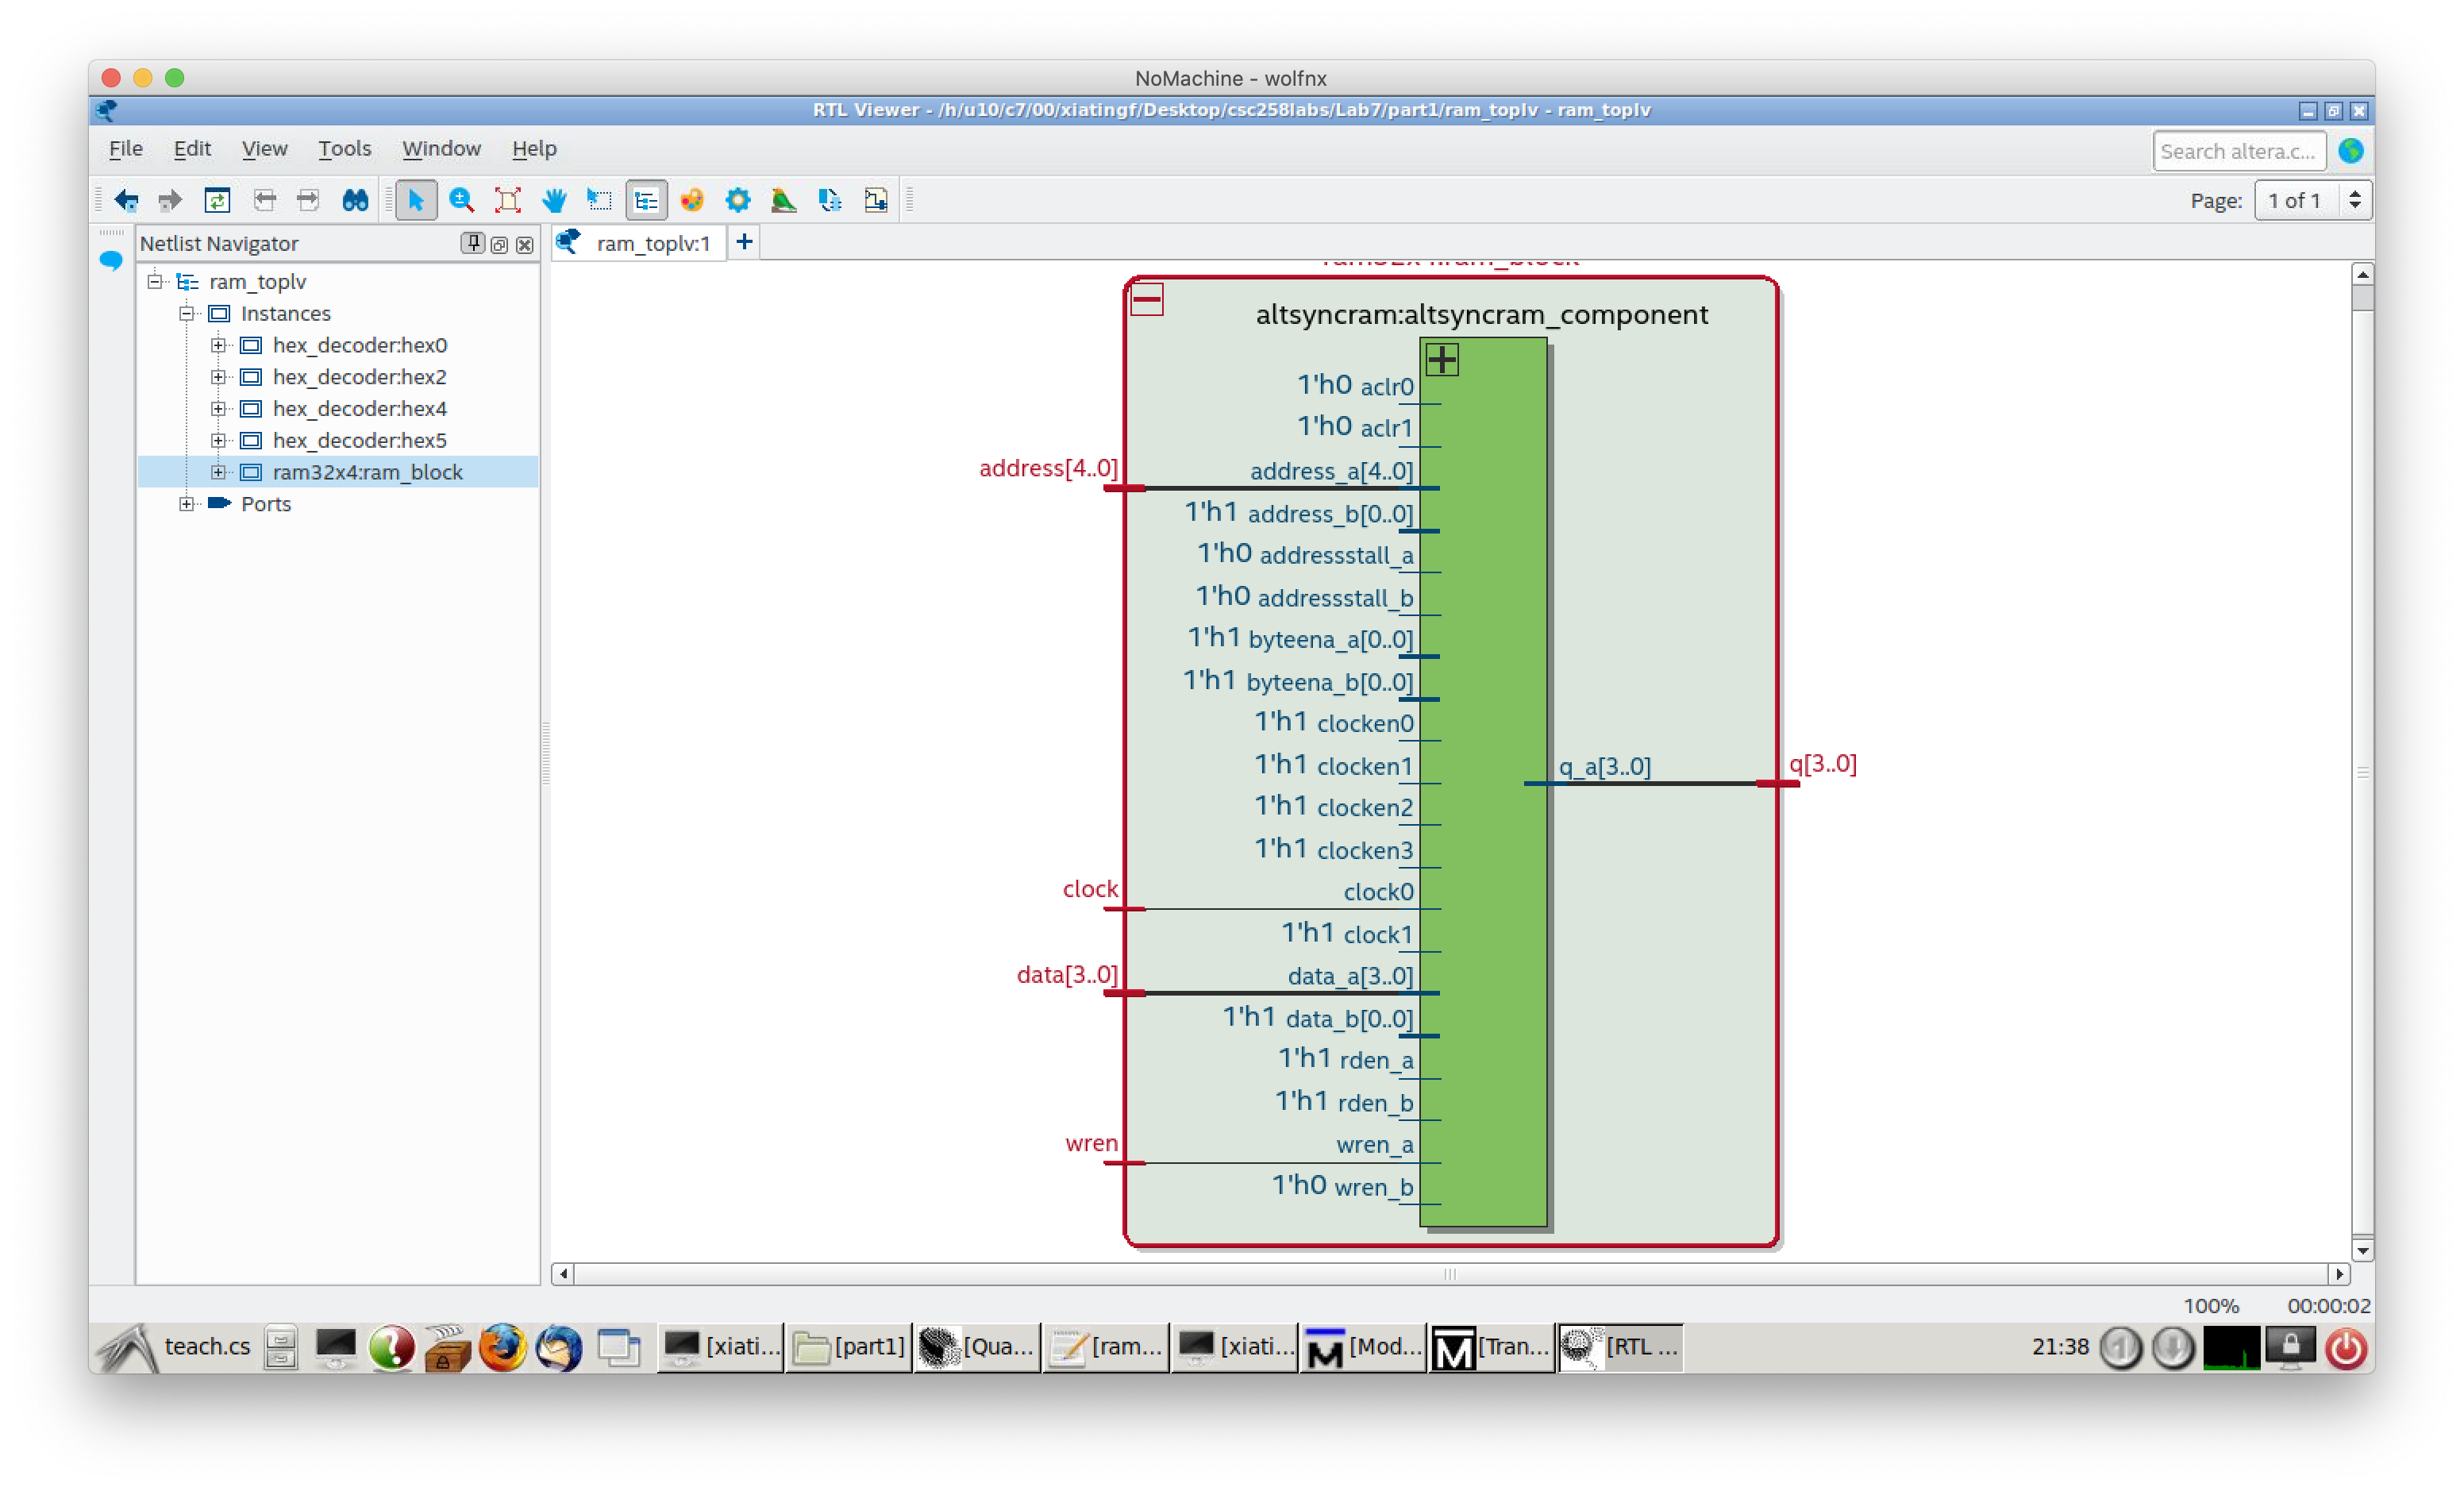
\includegraphics[scale=0.32]{part1_memory_block.png}
    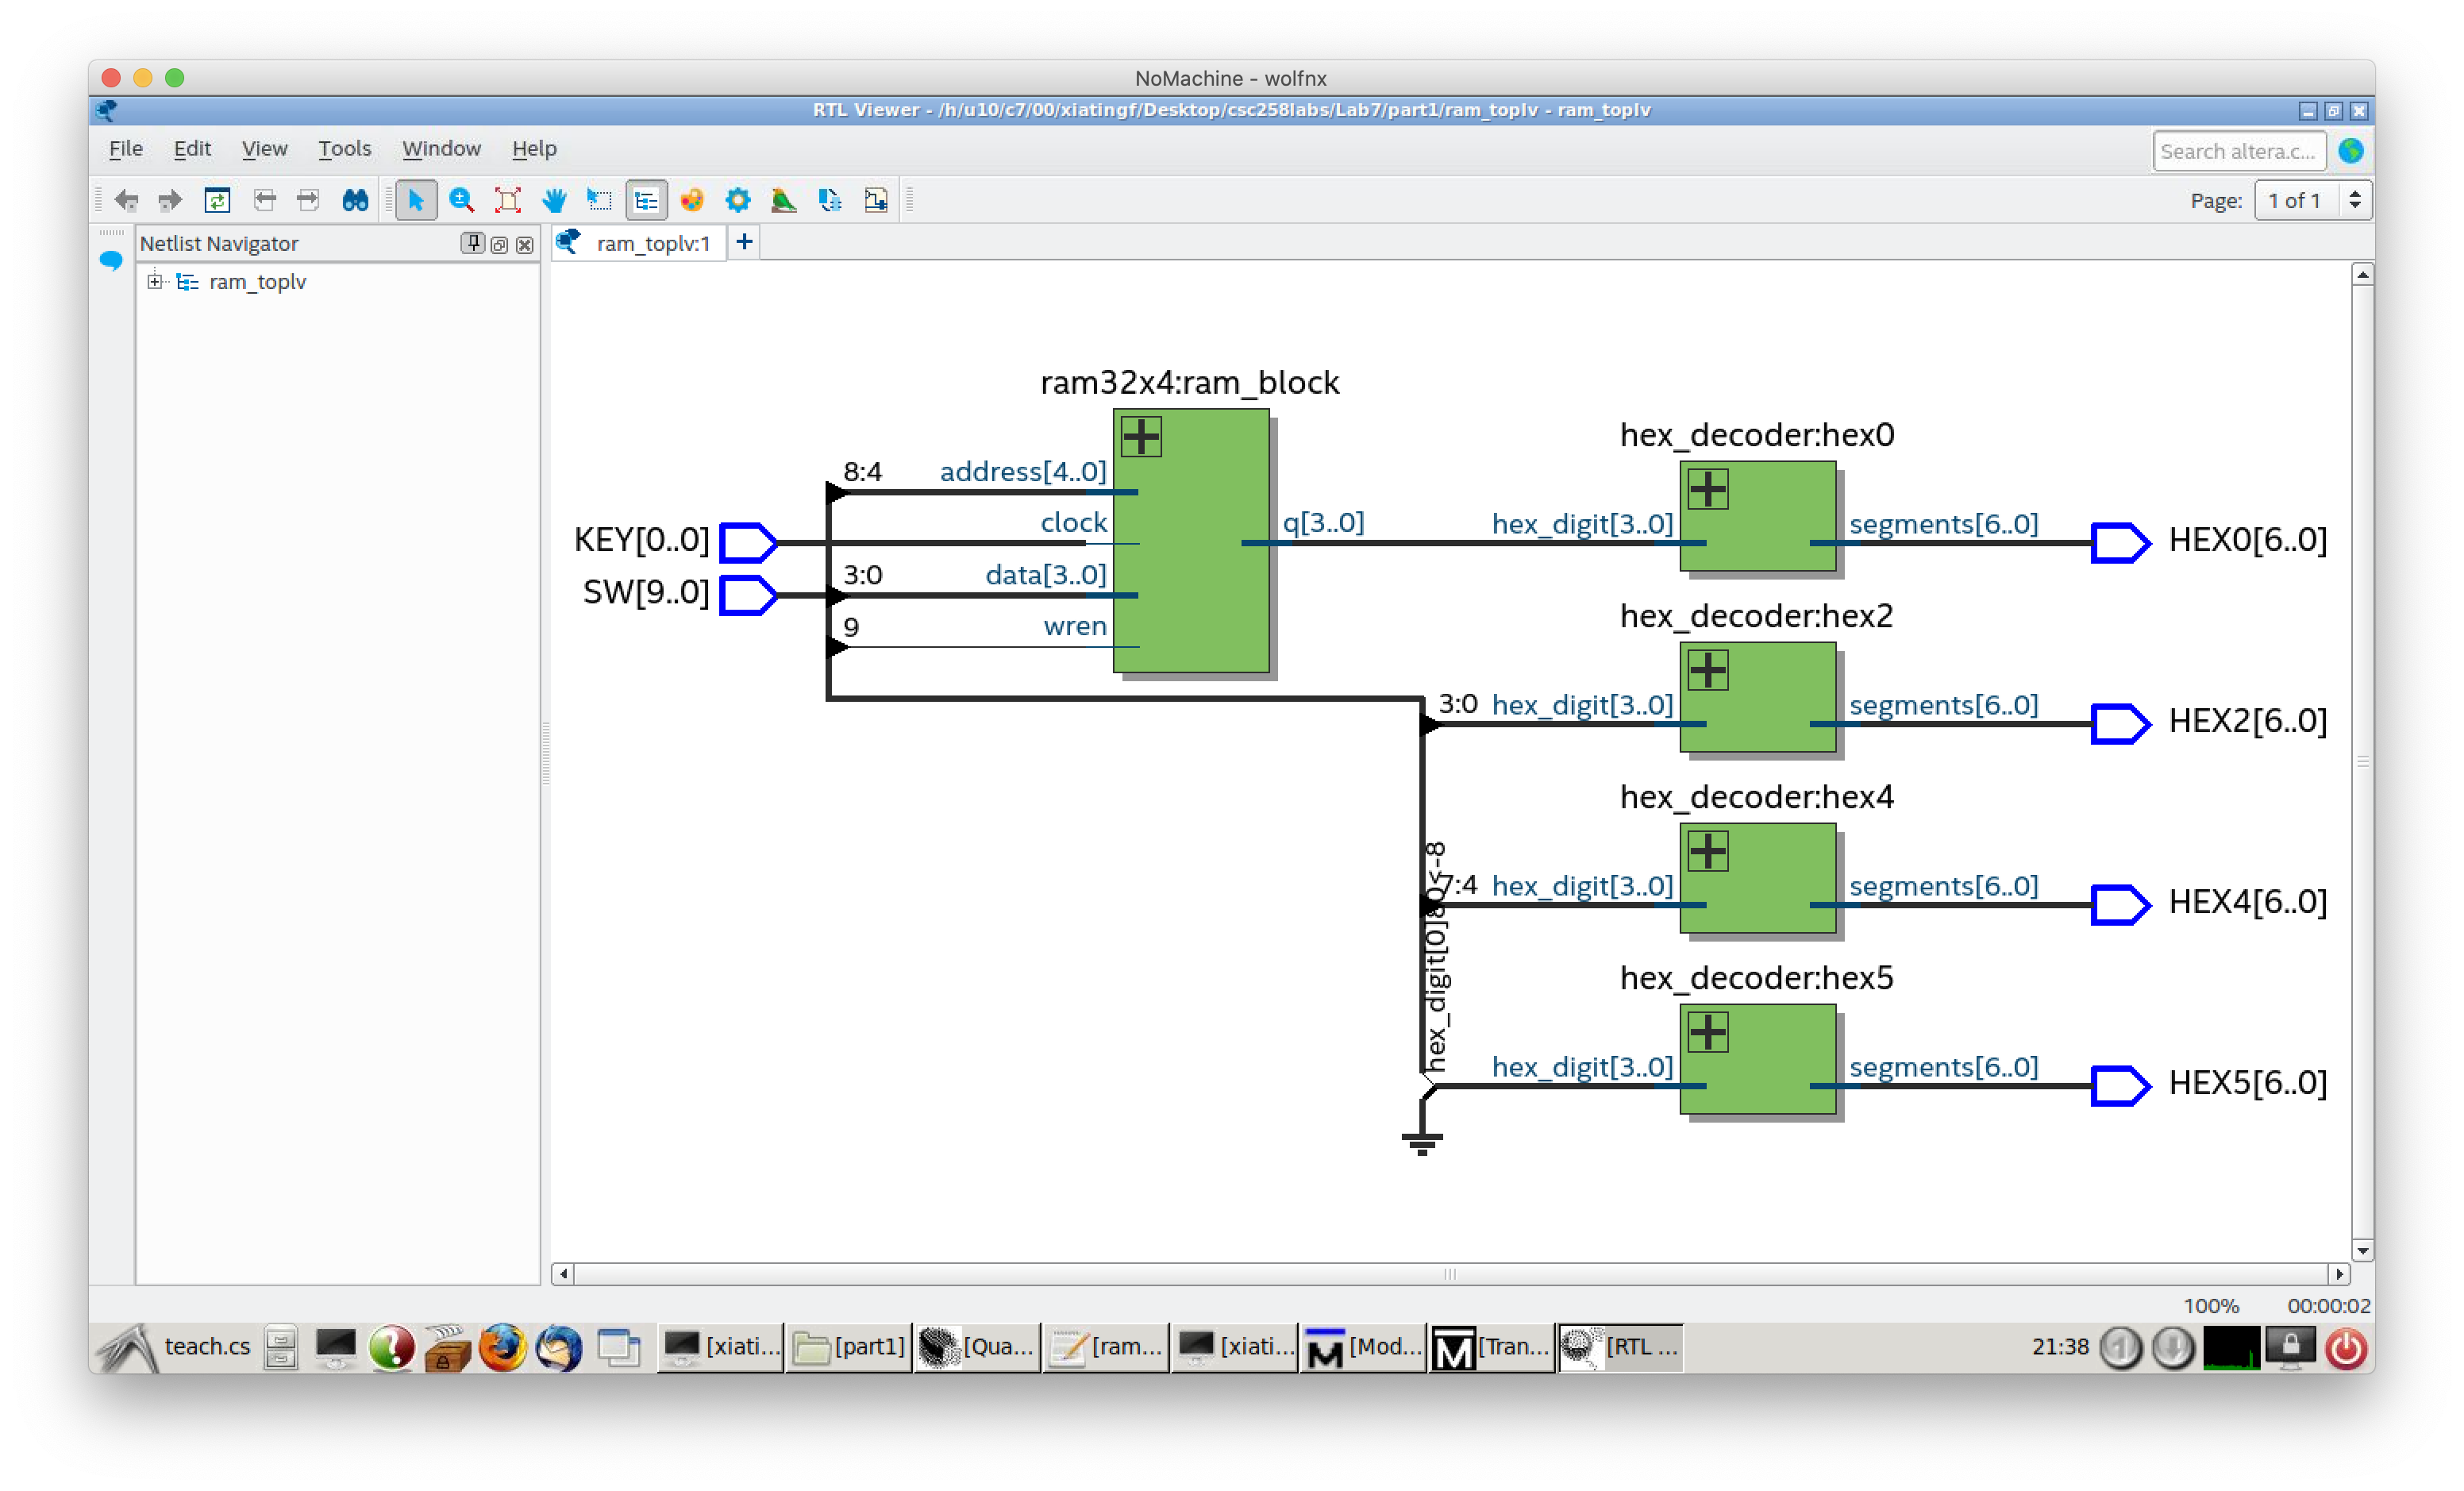
\includegraphics[scale=0.32]{part1_total_design.png}
\end{center}

\section*{PART II}
\paragraph{(1)} Here is my implementation of the datapath module
\begin{minted}{verilog}
    module datapath(
        input clk, resetn, ld_x, ld_y, ld_color,
        input [2:0] color_in,
        input [6:0] coordinate, 
        output [7:0] x_out, 
        output [6:0] y_out, 
        output [2:0] color_out
    );

        reg [7:0] x;
        reg [6:0] y;
        reg [2:0] color;
        reg [2:0] x_pos;
        reg [2:0] y_pos;

        //reset or load
        always @(posedge clk) begin
            if (!resetn) begin
                x <= 8'b0;
                y <= 7'b0;
                color <= 3'b0;
            end
            // the load signals tells if we are loading
            // or we are just printing the square
            else begin
                if (ld_x)
                    x <= {1'b0, coordinate};
                if (ld_y)
                    y <= coordinate;
                if (ld_color)
                    color <= color_in;
            end
        end
        //logic for  drawing the square
        always @(posedge clk) begin
            if (~resetn) begin
                x_pos <= 2'b00;
                y_pos <= 2'b00;
            end
            else
                if (x_pos == 2'b11 && y_pos == 2'b11) begin
                    x_pos <= 2'b00;
                    y_pos <= 2'b00;
                end
                else begin
                    if (x_pos == 2'b11) begin
                        x_pos <= 2'b00;
                        y_pos <= y_pos + 1'b1;
                    end 
                    else begin
                        x_pos <= x_pos + 1'b1;
                    end
                end
        end

        assign x_out = x + x_pos[1:0];
        assign y_out = y + y_pos[1:0];
        assign color_out = color;
    endmodule 
\end{minted}
Here is the ModelSim result for the datapath module, notice the box of size 4 by 4 is looped over in the \texttt{x\_out} and \texttt{y\_out} simulated.
\begin{center}
    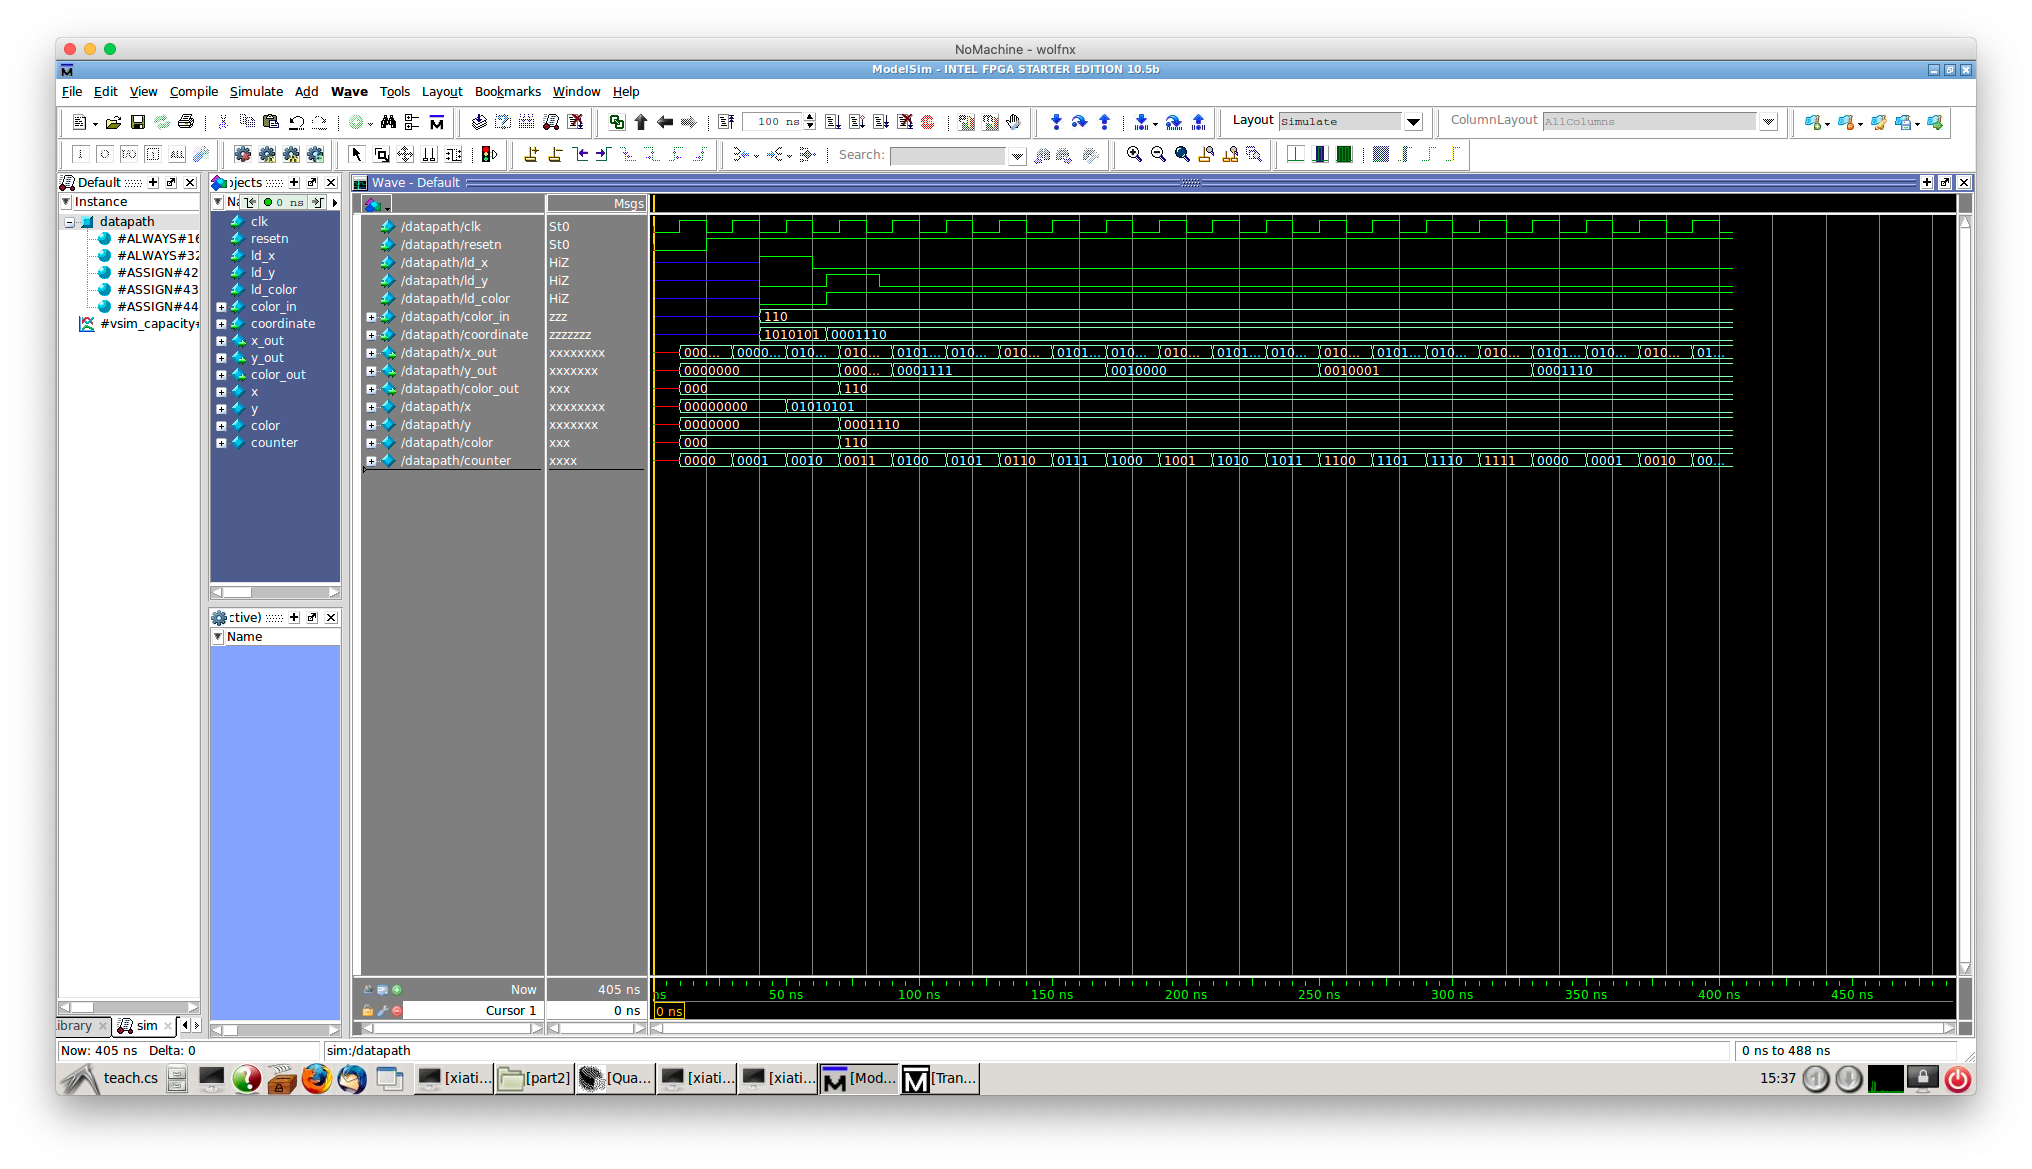
\includegraphics[scale=0.23]{part2_datapath_modelsim.png}
\end{center}
\paragraph{(2)} Here is my verilog module control, the FSM in the circuit
\begin{minted}{verilog}
    /// FSM module control, instantieation is c0
    module control(
        input clk, 
        input resetn, 
        input load, 
        input go,
        output reg ld_x, 
        output reg ld_y, 
        output reg ld_color, 
        output reg writeEn);

        reg [2:0] current_state, next_state;

        localparam  LOAD_X = 3'b000,
                        LOAD_X_WAIT = 3'b001,
                        LOAD_Y_C = 3'b010,
                        LOAD_Y_C_WAIT = 3'b011,
                        DO_PLOT = 3'b100;
        //reset
        always @(posedge clk) begin
            if (~resetn)
                current_state <= LOAD_X;
            else
                current_state <= next_state;
        end
        //state table
        always @(*) 
        begin: state_table
            case (current_state)
                LOAD_X: next_state = load ? LOAD_X_WAIT : LOAD_X;
                LOAD_X_WAIT: next_state = load ? LOAD_X_WAIT : LOAD_Y_C;
                LOAD_Y_C: next_state = go ? LOAD_Y_C_WAIT : LOAD_Y_C;
                LOAD_Y_C_WAIT: next_state = go ? LOAD_Y_C_WAIT : DO_PLOT;
                DO_PLOT: next_state = load ? LOAD_X : DO_PLOT;
                default: next_state = LOAD_X;
            endcase
        end

        always @(*)
        begin
            ld_x = 1'b0;
            ld_y = 1'b0;
            ld_color = 1'b0;
            writeEn = 0;
            case (current_state)
                LOAD_X: ld_x = 1;
                LOAD_X_WAIT: ld_x = 1;
                LOAD_Y_C: begin
                        ld_x = 0;
                        ld_y = 1;
                        ld_color = 1;
                end
                LOAD_Y_C_WAIT: begin
                        ld_x = 0;
                        ld_y = 1;
                        ld_color = 1;
                end
                DO_PLOT: writeEn = 1;
            endcase
        end
    endmodule
\end{minted}
Here is the screenshot for the ModelSim results for the FSM, notice the states incrementing and the \texttt{next\_state} is set as appropriate.
\begin{center}
    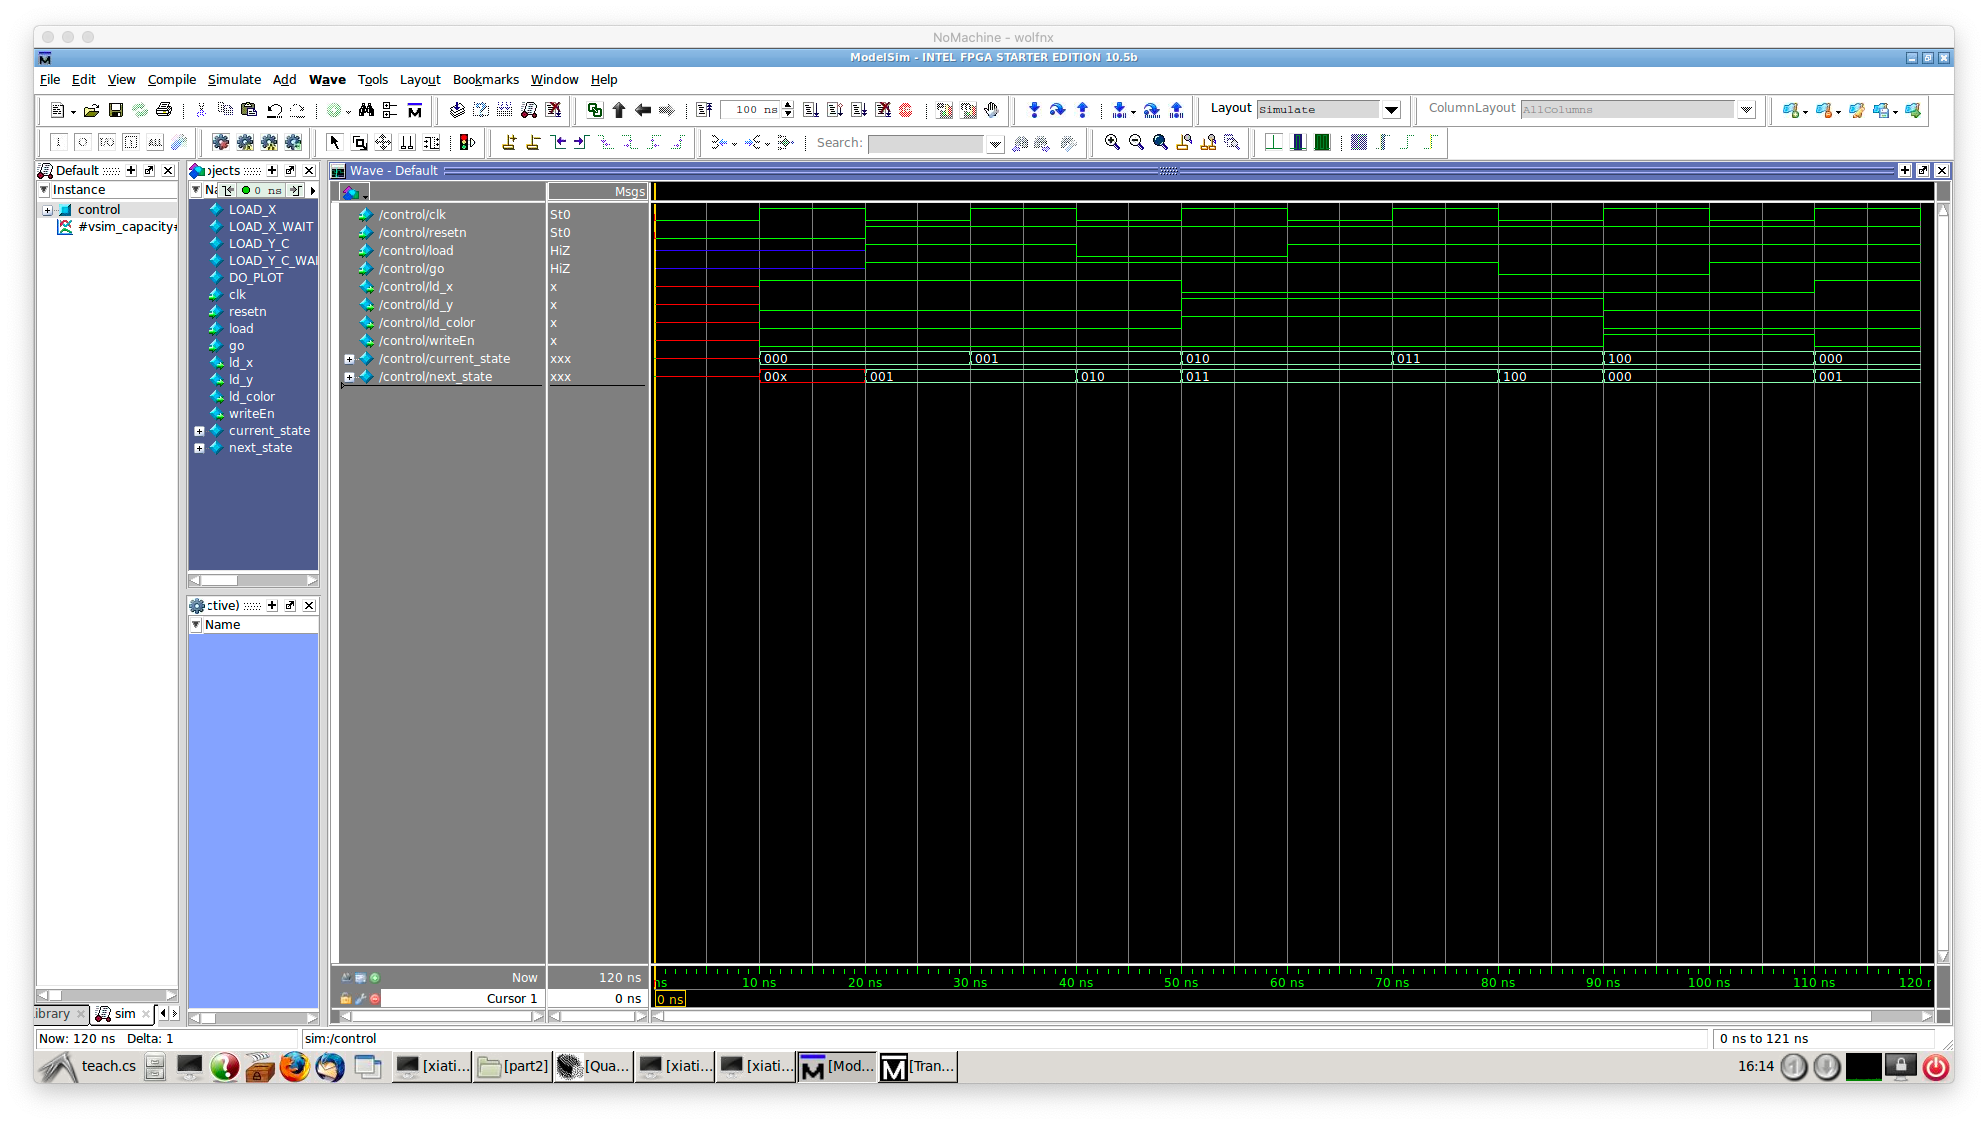
\includegraphics[scale=0.23]{part2_modelsim_control.png}
\end{center}

\paragraph{(c)} In the below code, I instantiated the \texttt{control} module and the \texttt{datapath} as approprate.
\begin{minted}{verilog}
    // Part 2 skeleton
    module part2
        (
            CLOCK_50,						//	On Board 50 MHz
            // Your inputs and outputs here
        KEY,
        SW,
            // The ports below are for the VGA output.  Do not change.
            VGA_CLK,   						//	VGA Clock
            VGA_HS,							//	VGA H_SYNC
            VGA_VS,							//	VGA V_SYNC
            VGA_BLANK_N,					//	VGA BLANK
            VGA_SYNC_N,						//	VGA SYNC
            VGA_R,   						//	VGA Red[9:0]
            VGA_G,	 						//	VGA Green[9:0]
            VGA_B   							//	VGA Blue[9:0]
        );

        input			CLOCK_50;				//	50 MHz
        input   [9:0]   SW;
        input   [3:0]   KEY;

        // Declare your inputs and outputs here
        // Do not change the following outputs
        output			VGA_CLK;   				//	VGA Clock
        output			VGA_HS;					//	VGA H_SYNC
        output			VGA_VS;					//	VGA V_SYNC
        output			VGA_BLANK_N;			//	VGA BLANK
        output			VGA_SYNC_N;				//	VGA SYNC
        output	[9:0]	VGA_R;   				//	VGA Red[9:0]
        output	[9:0]	VGA_G;	 				//	VGA Green[9:0]
        output	[9:0]	VGA_B;   				//	VGA Blue[9:0]
        
        wire resetn;
        assign resetn = KEY[0];
        
        // Create the colour, x, y and writeEn wires that are inputs to the controller.
        wire [2:0] colour;
        wire [7:0] x;
        wire [6:0] y;
        wire writeEn;

        // Create an Instance of a VGA controller - there can be only one!
        // Define the number of colours as well as the initial background
        // image file (.MIF) for the controller.
        vga_adapter VGA(
                .resetn(resetn),
                .clock(CLOCK_50),
                .colour(colour),
                .x(x),
                .y(y),
                .plot(writeEn),
                /* Signals for the DAC to drive the monitor. */
                .VGA_R(VGA_R),
                .VGA_G(VGA_G),
                .VGA_B(VGA_B),
                .VGA_HS(VGA_HS),
                .VGA_VS(VGA_VS),
                .VGA_BLANK(VGA_BLANK_N),
                .VGA_SYNC(VGA_SYNC_N),
                .VGA_CLK(VGA_CLK));
            defparam VGA.RESOLUTION = "160x120";
            defparam VGA.MONOCHROME = "FALSE";
            defparam VGA.BITS_PER_COLOUR_CHANNEL = 1;
            defparam VGA.BACKGROUND_IMAGE = "black.mif";
                
        // Put your code here. Your code should produce signals x,y,colour and writeEn/plot
        // for the VGA controller, in addition to any other functionality your design may require.
        
    // Instansiate datapath
        datapath d0(
            .clk(CLOCK_50),
            .color_in(SW[9:7]),
            .resetn(resetn),
            .ld_x(ld_x),
            .ld_y(ld_y),
            .ld_color(ld_color),
            .coordinate(SW[6:0]),
            .x_out(x),
            .y_out(y),
            .color_out(colour)
        );
        
    // Instansiate FSM control
    control c0(
            .clk(CLOCK_50),
            .resetn(resetn),
            .load(!(KEY[3])),
            .go(!(KEY[1])),
            .ld_x(ld_x),
            .ld_y(ld_y),
            .ld_color(ld_color),
            .writeEn(writeEn)	
        );

    endmodule

\end{minted}
\textbf{But some how model sim is complainning about missing modules when I try to simulate the above code, so I instantiated another module for the sake of testing the combination of FSM and datapath.} Here is the result of the simulation. 

\begin{center}
    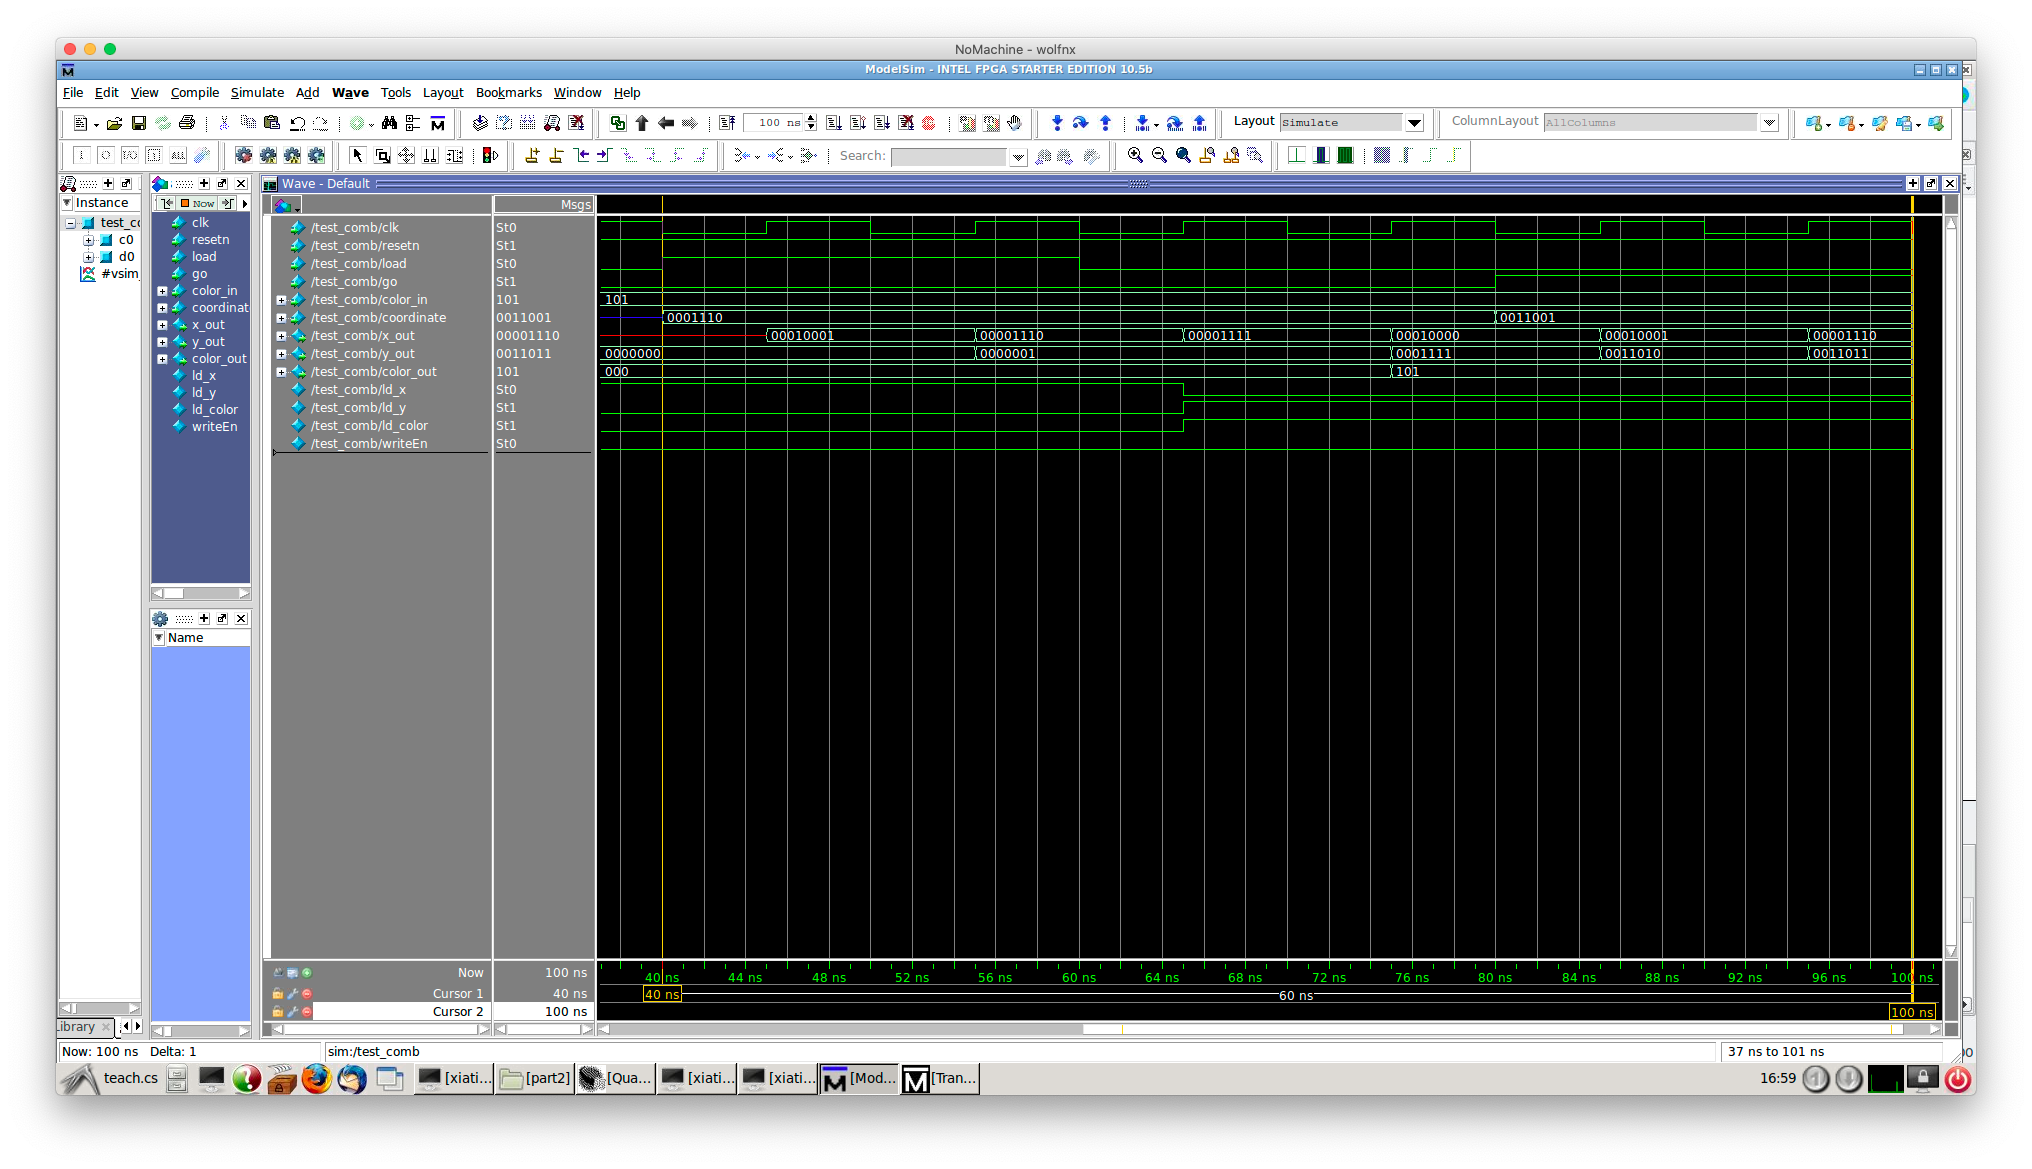
\includegraphics[scale=0.23]{part2_modelsim_test_comb.png}
\end{center}

Here is my code for this testing module

\begin{minted}{verilog}
    module test_comb(
        input clk, resetn, load, go,
        input [2:0] color_in,
        input [6:0] coordinate,
        output [7:0] x_out,
        output [6:0] y_out,
        output [2:0] color_out
        );

        wire ld_x, ld_y, ld_color, writeEn;

        control c0(
            .clk(clk),
            .resetn(resetn),
            .load(load),
            .go(go),
            .ld_x(ld_x),
            .ld_y(ld_y),
            .ld_color(ld_color),
            .writeEn(writeEn)	
        );

        datapath d0(
            .clk(clk),
            .color_in(color_in[2:0]),
            .resetn(resetn),
            .ld_x(ld_x),
            .ld_y(ld_y),
            .ld_color(ld_color),
            .coordinate(coordinate[6:0]),
            .x_out(x_out),
            .y_out(y_out),
            .color_out(color_out)
        );
        
    endmodule
\end{minted}

\section*{PART III}


\end{document}
